\chapter{Creating New Boards}


\section{How to Compile PICsimLab}

\subsection{In Debian Linux and derivatives}

 \begin{minted}[baselinestretch=1.2,fontsize=\footnotesize,bgcolor=colorbash]{bash}
git clone https://github.com/lcgamboa/picsimlab.git
cd picsimlab
./picsimlab_build_all_and_deps.sh
\end{minted}

To build experimental version use the argument ``exp'' with the \textit{picsimlab\_build\_all\_and\_deps.sh} script


\subsection{Cross-compiling for windows} 

For Windows 64 bits version from Debian Linux and derivatives or \href{https://docs.microsoft.com/windows/wsl/install-win10}{WSL} (Windows Subsystem for Linux ) on win10

\begin{minted}[baselinestretch=1.2,fontsize=\footnotesize,bgcolor=colorbash]{bash}
git clone https://github.com/lcgamboa/picsimlab.git
cd picsimlab
./picsimlab_build_w64.sh
\end{minted}

For 32 bits version:

\begin{minted}[baselinestretch=1.2,fontsize=\footnotesize,bgcolor=colorbash]{bash}
git clone https://github.com/lcgamboa/picsimlab.git
cd picsimlab
./picsimlab_build_w32.sh
\end{minted}

To build experimental version use the argument ``exp'' with the scripts.


% Code to compile:
% \begin{itemize}
%  \item  liblxrad (lxrad.dll)
%  \item  libpicsim (picsim.dll)
%  \item  PicsimLab (picsimlab.exe)
% \end{itemize}
% 
% 
% Tools needed:
% \begin{itemize}
%  \item make
%  \item gcc
%  \item g++
%  \item autoconf
%  \item doxygen 
% \end{itemize}
% 
% Dependencies:
% \begin{itemize}
%  \item wxwidgets-3.0 
% \end{itemize}
% 
% 
% \subsection{Install Compilers and Tools}
% 
% 
% For Linux based in debian distro:
% 
% \begin{minted}[baselinestretch=1.2,fontsize=\footnotesize,bgcolor=colorbash]{bash}
% sudo apt-get install make gcc g++ autoconf doxygen libwxgtk3.0-dev 
% \end{minted}
% 
% 
% For Windows: 
% \begin{itemize}
%  \item Install \href{http://www.mingw.org/wiki/msys}{MinGW MSYS} 
%  \item Download and compile \href{http://www.wxwidgets.org/}{wxwidgets-3.0}  with MSYS.
% \end{itemize}
% 
% \subsection{Compiling and Install LXRAD Library}
% 
% Link for source code download \href{http://sourceforge.net/projects/lxrad/files/lxrad/lxrad-0.8_wx/lxrad-0.8.tgz/download}{lxrad-0.8.tgz}. 
% 
% To build lxrad, open a shell (MSYS in windows) and type the following commands in the folder of downloaded file:
% 
% \begin{minted}[baselinestretch=1.2,fontsize=\footnotesize,bgcolor=colorbash]{bash}
% tar xvfz lxrad-0.8.tgz <enter>
% cd lxrad-0.8 <enter>
% autoconf <enter>
% ./configure <enter>
% make <enter>
% sudo make install <enter> 
% \end{minted}
% 
% 
% \subsection{Compiling and Install PICsim Library}
% 
% Link for source code download \href{http://sourceforge.net/projects/picsim/files/picsim/picsim-0.6/picsim-0.6.tgz/download}{picsim-0.6.tgz}. 
% 
% To build picsim library, open a shell (MSYS in windows) and type the following commands in the folder of downloaded file:
% 
% \begin{minted}[baselinestretch=1.2,fontsize=\footnotesize,bgcolor=colorbash]{bash}
% tar xvfz picsim-0.6.tgz <enter>
% cd picsim-0.6 <enter>
% make <enter>
% sudo make install <enter>
% sudo ldconfig <enter>
% \end{minted}
% 
% \subsection{Compiling and Install PICsimLab}
% 
% Link for source code download \href{http://sourceforge.net/projects/picsim/files/picsim/picsim-0.6/picsimlab-0.6.tgz/download}{PICsimLab-0.6}. 
% 
% To build PICsimLab, open a shell (MSYS in windows) and type the following commands in the folder of downloaded file:
% 
% \begin{minted}[baselinestretch=1.2,fontsize=\footnotesize,bgcolor=colorbash]{bash}
% tar xvfz picsimlab-0.6.tgz <enter>
% cd picsimlab-0.6 <enter> 
% make <enter>
% sudo make install <enter>
% \end{minted}
% 
% You can use \href{https://netbeans.org/downloads/}{netbeans IDE} with C/C++ plugin to compile PICsimLab using \href{http://www.mingw.org/wiki/msys}{MSYS}. 
% After extract files, open netbeans and create a C/C++ project using existing files and search for picsimlab-0.6 directory. 

\section{Creating a New Board}

The first step is get the schematic and all information about the board hardware.
The second step is the creation of five files in PICSimLab dir (consider replace the 'x' of board\_x for a number or name in your case):
\begin{itemize}
\item Board Picture (share/boards/x/board.png);
\item Board input map (share/boards/x/input.map);
\item Board output map (share/boards/x/output.map);
\item Board header (src/boards/board\_x.h);
\item Board C++ code (src/boards/board\_x.cc);
\end{itemize}

The third and last step is recompiling PICSimLab with new board support.

\subsection{Board Hardware and Schematic}

For this tutorial, the board created have the hardware shown in diagram below:
\begin{figure}[H]
\center
\includegraphics[width=0.7\textwidth]{img/hb/blocks.eps} 
\end{figure} 

The schematic for the tutorial board made in \href{http://kicad-pcb.org/}{Kicad}.
\begin{figure}[H]
\center
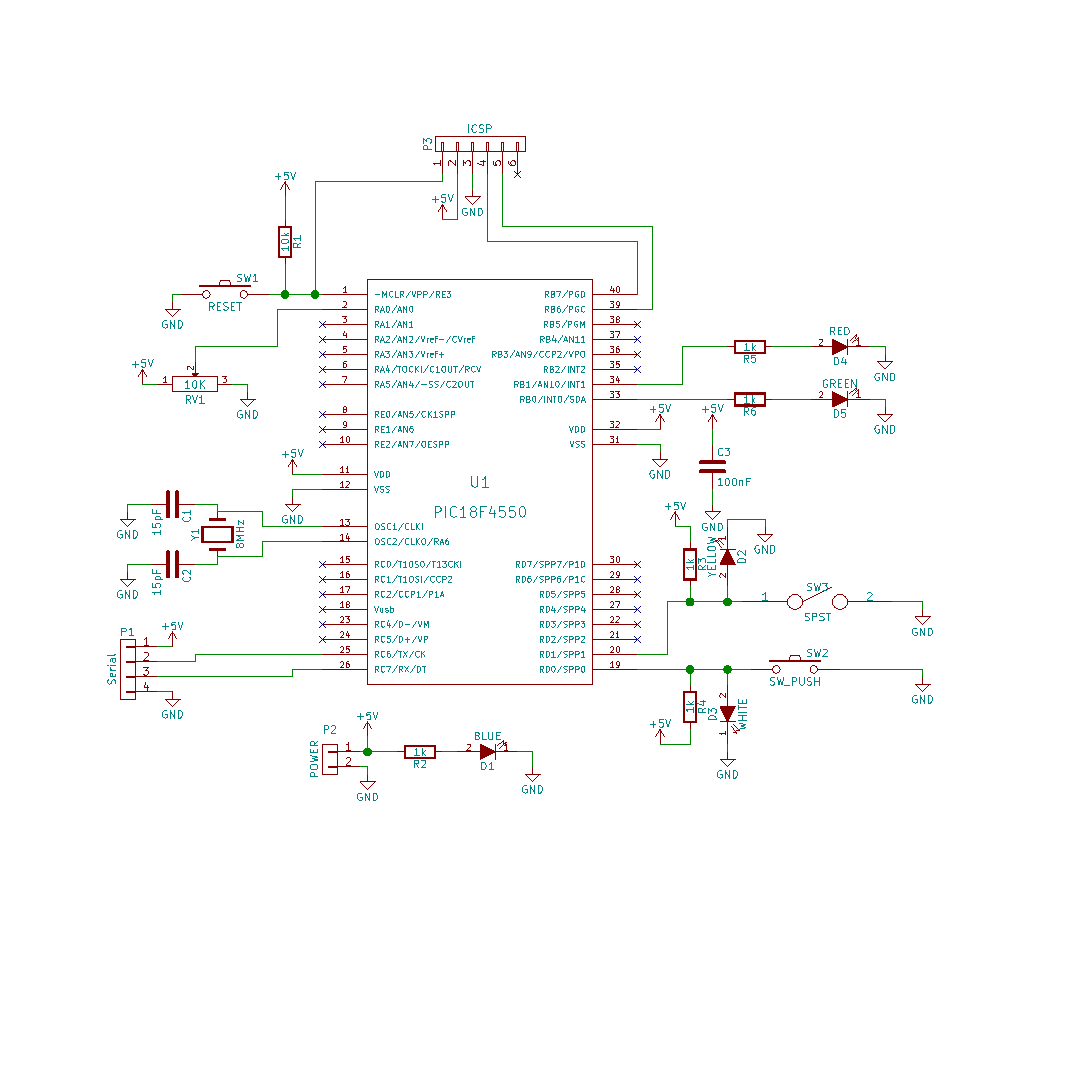
\includegraphics[width=0.99\textwidth]{board_x/board_x.eps} 
\end{figure} 

\pagebreak
And the PCB layout was made in \href{http://kicad-pcb.org/}{Kicad} too. The PCB is not necessary if you have a real board.

\begin{figure}[H]
\center
\includegraphics[width=0.9\textwidth, angle=-90]{board_x/board_x_pcb.eps} 
\end{figure} 

\pagebreak
\subsection{Board Picture}


Because the real board of this tutorial never has been built, the board picture was taken from \href{http://kicad-pcb.org/}{Kicad} 3D viewer.
The picture image is saved as ``share/board/x/board.png''.

\begin{figure}[H]
\center
\includegraphics[width=0.8\textwidth]{files/share/board.png} 
\end{figure} 

It is also possible to use images in SVG format for better viewing quality. \href{https://github.com/yaqwsx/PcbDraw}{PCBDraw} can be used to convert a Kicad PCB project to 
an SVG image. 

\begin{figure}[H]
\center
\includegraphics[width=0.8\textwidth]{files/share/board_svg.png} 
\end{figure} 

\pagebreak
\subsection{Picture maps}
The PICSimLab use two type of image maps. 
The input map mark the areas in board picture which user can interact (by mouse click). 
The output map mark the areas in board picture to be redraw according simulator status. 
The picture maps used for PICSimLab are normal HTML image-map. They can be made by hand or using any software which can handle image maps. The original PICSimLab maps are made using \href{http://www.gimp.org/}{Gimp image editor}.     

To start, in the GIMP, use the Filters->Web->Image Map to open image map editor window.
\begin{figure}[H]
\center
\includegraphics[width=0.99\textwidth]{img/hb/gimp01.png} 
\end{figure} 

\pagebreak
Then select rectangle or circle map on toolbar.
\begin{figure}[H]
\center
\includegraphics[width=0.8\textwidth]{img/hb/gimp02.png} 
\end{figure} 

And mark the area in picture.
\begin{figure}[H]
\center
\includegraphics[width=0.8\textwidth]{img/hb/gimp03.png} 
\end{figure} 

\pagebreak
After area is select, in the settings windows select the link type for ``Other''. 
\begin{figure}[H]
\center
\includegraphics[width=0.7\textwidth]{img/hb/gimp04.png} 
\end{figure} 

And write the name of area. The name must describe the area function on the board.
\begin{figure}[H]
\center
\includegraphics[width=0.7\textwidth]{img/hb/gimp05.png} 
\end{figure} 


\subsubsection{Board map}

For this tutorial board, five input areas are marked:
\begin{itemize}
\item I\_ICSP - where user click to load hexfile.
\item I\_PWR - where user click to turn on/off the board.
\item I\_RST - Button to reset board.
\item I\_D0 - Button connected in RD0. 
\item I\_D1 - Switch connected in RD1.
\end{itemize}

For this tutorial board, six output areas are marked:
\begin{itemize}
\item O\_SD1 - draw the switch on/off.
\item O\_LD0 - draw LED connected in button.
\item O\_LD1 - draw LED connected in switch.
\item O\_LPWR - draw power LED indicator.
\item O\_RB0 and O\_RB1 - draw LEDs connected in RB0 and RB1.
\end{itemize}


\begin{figure}[H]
\center
\includegraphics[width=0.7\textwidth]{img/hb/gimp06.png} 
\end{figure} 

\begin{figure}[H]
\center
\includegraphics[width=0.7\textwidth]{img/hb/gimp07.png} 
\end{figure} 

Board map generated by Gimp image map editor and saved as ``share/boards/X/board.map''.
\inputminted[baselinestretch=1.2,fontsize=\footnotesize,linenos]{html}{files/share/board.map}

The kicad project files can be download from github \href{https://github.com/lcgamboa/picsimlab/tree/master/docs/kicad/board_x}{PICSimLab repository}. 

\subsection{Board code}

The header file and c++ code file with comments are listed in the next two subsections. This files control the behavior of board in simulator.

\subsubsection{board\_x.h}

\href{https://github.com/lcgamboa/picsimlab/blob/master/src/boards/board_x.h}{ board\_x.h online file}.

\href{https://lcgamboa.github.io/picsimlab/devel/html/index.html#binc}{ board\_x.h online doxygen version}.


\inputminted[baselinestretch=1.2,fontsize=\footnotesize,linenos]{c++}{files/board_x.h}

\pagebreak
\subsubsection{board\_x.cc}

\href{https://github.com/lcgamboa/picsimlab/blob/master/src/boards/board_x.cc}{ board\_x.cc online file}.

\href{https://lcgamboa.github.io/picsimlab/devel/html/index.html#bcode}{ board\_x.cc online doxygen version}.

\inputminted[baselinestretch=1.2,fontsize=\footnotesize,linenos]{c++}{files/board_x.cc}


\subsection{Integration with PICsimLab}

To integration of the new board in PICSimLab, are necessary edit one file.

The file is Makefile.Common. The only change to be made is include object \textbf{boards/board\_board\_x.o} in 
 objects list. They can be added in variable OBJS or OBJS\_EXP (used only in experimental version).

After change the Makefile.Common and include the five files created for new board, the PICSimLab can be recompiled, as described in first chapter.


\subsection{Final Result}

The PICSimLab board created for this tutorial are shown in the figure below.
\begin{figure}[H]
\center
\includegraphics[width=0.9\textwidth]{img/hb/final.png} 
\end{figure} 

The sample program below can be used to test new board, this code is write for XC8 compiler:
\inputminted[baselinestretch=1.2,fontsize=\footnotesize,linenos]{c}{sample/board_x.c}

